\documentclass{beamer}

\usepackage{listings}
\usepackage{color}
\usepackage{alltt}
\usepackage{graphicx}




\title 
{Applying Panel Data Methods to Other Data Structures}
\author
{Professor Jan Minx}
\institute
{Hertie School of Governance}
\date
{Stats II, Lecture ?, ? 2015}

\begin{document}

  \frame{\titlepage}

  \begin{frame}
    \frametitle{Applying Panel Data Methods to Other Data Structures}
    \framesubtitle{Motivation}
    \begin{itemize}
      \item Panel data methods can be used with data structures that do not involve time
      \item Hierarchical data structures contain clusters of observation which share common characteristics
      \item When these characteristics are unobservable and correlated with other explanatory variables, pooled OLS will give us estimates that are biased and inefficient
    \end{itemize}
  \end{frame}
  
  \begin{frame}
    \frametitle{Applying Panel Data Methods to Other Data Structures}
    \framesubtitle{Motivation}
    \begin{itemize}
      \item Consider a geographical dataset that observes variables for small areas (in this case MSOAs, 
      or Middle Layer Super Output Areas)
      \item Each small area belongs to a local authority
      \item If local authority attributes that we cannot observe affect our other variables, we will get biased and inefficient estimates using OLS
    \end{itemize}
  \end{frame}
  
  \begin{frame}
    \frametitle{Applying Panel Data Methods to Other Data Structures}
    \framesubtitle{Motivation}
    Remember that OLS regression is estimated using the equation
    $$ y_{i} = \beta_{0} + \beta_{1}x_{i} + u_{i} $$
    
    When we use panel methods across time, our equation becomes
    $$ y_{it} = \beta_{0} + \beta_{1}x_{it} + a_{i} + u_{it} $$
    Here the variable $a_{i}$ captures all unobserved, time-constant factors that affect $y_{it}$
  \end{frame}
    
  \begin{frame}
    \frametitle{Applying Panel Data Methods to Other Data Structures}
    \framesubtitle{Motivation}
    
    By constructing our dataset and a fixed effects model carefully, we can also account for fixed effects given by local authorities with the equation
    $$ y_{pc} = \beta_{0} + \beta_{1}x_{pc} + a_{p} + u_{pc} $$
    where, given our hierarchical data structure, $p$ indexes the parent (local authority) and $c$ indexes the child (MSOA)
    
    \bigskip
    
    Here the local authority fixed effect is given by $a_{p}$, and the coefficient $\beta_{1}x_{pc}$ describes the effect of our explanatory variable on our independent variable $x$ \textit{within} local authorities.
    
  \end{frame}
  
  \begin{frame}
    \frametitle{Applying Panel Data Methods to Other Data Structures}
    \framesubtitle{Pooled OLS}
    When we use a pooled OLS regression on our dataset to estimate the effect of income on household energy consumption, we get the following results
    \tiny
    \begin{alltt}
    reg energy\_consumption income\_est
    
    outtex, file(ols.tex) labels level detail legend key(stab) replace
    est store ols
    \end{alltt}

    
{
\def\onepc{$^{\ast\ast}$} \def\fivepc{$^{\ast}$}
\def\tenpc{$^{\dag}$}
\def\legend{\multicolumn{4}{l}{\footnotesize{Significance levels
:\hspace{1em} $\dag$ : 10\% \hspace{1em}
$\ast$ : 5\% \hspace{1em} $\ast\ast$ : 1\% \normalsize}}}
\begin{table}[htbp]\centering
 \caption{Estimation results : regress
\label{stab}}
\begin{tabular}{l r @{} l c }\hline\hline 
\multicolumn{1}{c}
{\textbf{Variable}}
 & \multicolumn{2}{c}{\textbf{Coefficient}}  & \textbf{(Std. Err.)} \\ \hline
income\_est  &  11.681&\onepc  & (0.222)\\
Intercept  &  16142.067&\onepc  & (139.382)\\
\hline\multicolumn{4}{c}{}\\
\hline N & \multicolumn{3}{c}{7133}\\
R$^{2}$ & \multicolumn{3}{c}{0.28}\\
F $ _{(1,7131)}$ & \multicolumn{3}{c}{2766.551}\\
\hline\legend
\end{tabular}
\end{table}
}


  \end{frame}
  
  \begin{frame}
    \frametitle{Applying Panel Data Methods to Other Data Structures}
    \framesubtitle{Pooled OLS}
    \tiny
    \begin{alltt}
    graph twoway (scatter energy\_consumption income\_est) ///
    
    (lfit energy\_consumption income\_est)
    \end{alltt}
    
    \begin{figure}
    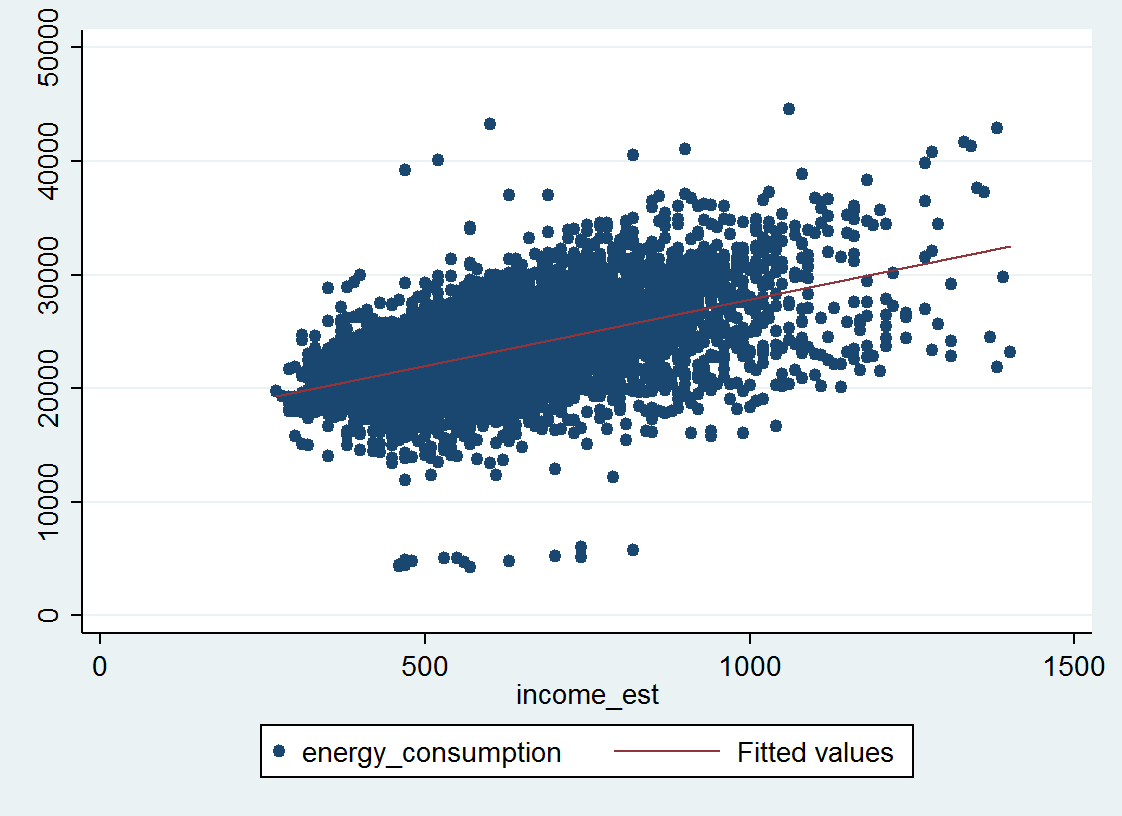
\includegraphics[width=8cm]{../stata_code/ols.png}
    \centering
    \end{figure}
  \end{frame}
  
  \begin{frame}
    \frametitle{Applying Panel Data Methods to Other Data Structures}
    \framesubtitle{Fixed Effects}
    When we use a fixed effects model to estimate the effect of income on household energy consumption \textit{within} local authorities, the size of the effect changes.
    \tiny
    \begin{alltt}
    xtset LA\_CODE MSOA\_CODE
    
    xtreg energy\_consumption income\_est, fe
    
    outtex, file(fe.tex) labels level detail legend key(stab) replace
    
    est store fe
    \end{alltt}
    
    
    
{
\begin{table}[htbp]\centering
 \caption{Estimation results : xtreg
\label{tabresult xtreg}}
\begin{tabular}{l c c }\hline\hline 
\multicolumn{1}{c}
{\textbf{Variable}}
 & {\textbf{Coefficient}}  & \textbf{(Std. Err.)} \\ \hline
income\_est  &  20.111  & (0.237)\\
Intercept  &  11040.143  & (145.751)\\
\hline\end{tabular}
\end{table}
}


  \end{frame}
  
  \begin{frame}
    \frametitle{Applying Panel Data Methods to Other Data Structures}
    \framesubtitle{Fixed Effects}
    \tiny
    \begin{alltt}
xi: regress energy\_consumption income\_est i.LA\_CODE

predict energy\_consumption\_fitted

separate energy\_consumption, by(LA\_CODE)

separate energy\_consumption\_fitted, by(LA\_CODE)

graph twoway (scatter energy\_consumption1-energy\_consumption80 income\_est) ///
	
	(line energy\_consumption\_fitted1-energy\_consumption\_fitted80 income\_est) ///
	
	(lfit energy\_consumption income\_est, ///
	
	color(black) lwidth(thick) lpattern(dash)), legend(off) , legend(off) 
    \end{alltt}
    
    \begin{figure}
    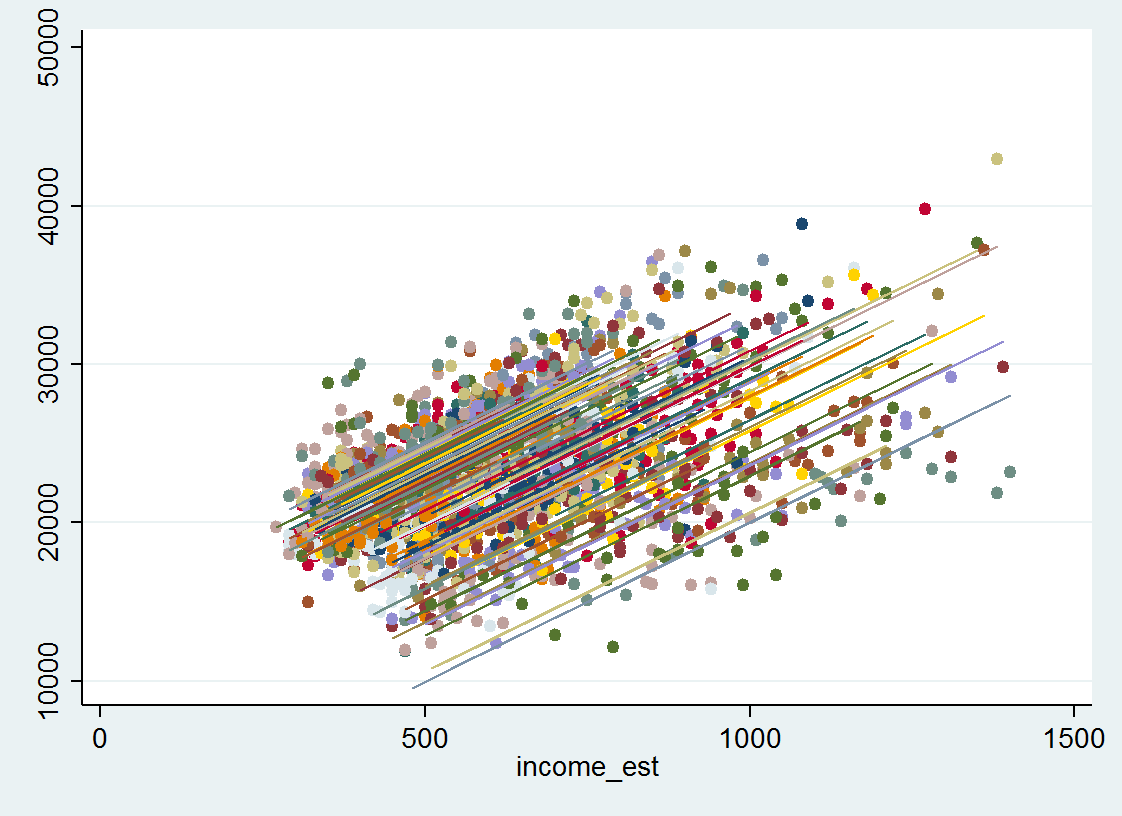
\includegraphics[width=8cm]{../stata_code/fe.png}
    \centering
    \end{figure}
  \end{frame}
  
  \begin{frame}
    \frametitle{Applying Panel Data Methods to Other Data Structures}
    \framesubtitle{Comparing OLS with Fixed Effects Models}
    \tiny
    \begin{alltt}
      esttab ols fe using table1.tex, replace
    \end{alltt}
    \small
    {
\def\sym#1{\ifmmode^{#1}\else\(^{#1}\)\fi}
\begin{tabular}{l*{2}{c}}
\hline\hline
            &\multicolumn{1}{c}{(1)}&\multicolumn{1}{c}{(2)}\\
            &\multicolumn{1}{c}{energy\_consumption}&\multicolumn{1}{c}{energy\_consumption}\\
\hline
income\_est  &       11.68\sym{***}&       20.11\sym{***}\\
            &     (52.60)         &     (84.86)         \\
[1em]
\_cons      &     16142.1\sym{***}&     11040.1\sym{***}\\
            &    (115.81)         &     (75.75)         \\
\hline
\(N\)       &        7133         &        7133         \\
\hline\hline
\multicolumn{3}{l}{\footnotesize \textit{t} statistics in parentheses}\\
\multicolumn{3}{l}{\footnotesize \sym{*} \(p<0.05\), \sym{**} \(p<0.01\), \sym{***} \(p<0.001\)}\\
\end{tabular}
}

    
  \end{frame}

\end{document}